% Created 2021-05-03 lun. 11:24
% Intended LaTeX compiler: pdflatex
\documentclass[11pt]{article}
\usepackage[utf8]{inputenc}
\usepackage[T1]{fontenc}
\usepackage{graphicx}
\usepackage{grffile}
\usepackage{longtable}
\usepackage{wrapfig}
\usepackage{rotating}
\usepackage[normalem]{ulem}
\usepackage{amsmath}
\usepackage{textcomp}
\usepackage{amssymb}
\usepackage{capt-of}
\usepackage{hyperref}
\usepackage{color}
\usepackage{mathpazo}
\usepackage[natbibapa]{apacite}
\author{Frédéric Santos}
\date{\today}
\title{pacmanUB : un clone de pacman made in Bordeaux}
\hypersetup{
 pdfauthor={Frédéric Santos},
 pdftitle={pacmanUB : un clone de pacman made in Bordeaux},
 pdfkeywords={},
 pdfsubject={},
 pdfcreator={Emacs 27.2 (Org mode 9.4.5)}, 
 pdflang={French}}
\begin{document}

\maketitle
\tableofcontents


\section{Présentation du logiciel}
\label{sec:orgf71e721}
Lorem ipsum dolor sit amet, consectetuer adipiscing elit.  Donec hendrerit tempor tellus.  Donec pretium posuere tellus.  Proin quam nisl, tincidunt et, mattis eget, convallis nec, purus.  Cum sociis natoque penatibus et magnis dis parturient montes, nascetur ridiculus mus.  Nulla posuere.  Donec vitae dolor.  Nullam tristique diam non turpis.  Cras placerat accumsan nulla.  Nullam rutrum.  Nam vestibulum accumsan nisl.

\section{Installation}
\label{sec:org555d520}
\subsection{Linux}
\label{sec:org2088372}
\subsection{Mac OS}
\label{sec:org7c59971}
Lorem ipsum dolor sit amet, consectetuer adipiscing elit.  Donec hendrerit tempor tellus.  Donec pretium posuere tellus.  Proin quam nisl, tincidunt et, mattis eget, convallis nec, purus.  Cum sociis natoque penatibus et magnis dis parturient montes, nascetur ridiculus mus.  Nulla posuere.  Donec vitae dolor.  Nullam tristique diam non turpis.  Cras placerat accumsan nulla.  Nullam rutrum.  Nam vestibulum accumsan nisl.

\subsection{Windows}
\label{sec:org9090ab3}
\subsubsection{Windows 7}
\label{sec:org04bcdcb}
\begin{itemize}
\item Télécharger
\item Décompresser
\item Installer
\end{itemize}

\subsubsection{Windows 10}
\label{sec:org95f8092}
\begin{enumerate}
\item Télécharger
\item Décompresser
\item Installer
\end{enumerate}

\section{Comparaison avec d'autres logiciels}
\label{sec:orgcc592eb}
Les autres Pacman disponibles sont décrits en table \ref{tab-concurrence}.

\begin{table}[htbp]
\centering
\begin{tabular}{llr}
\hline
Logiciels & OS & Prix\\
\hline
pacmanUB & Tous les OS & 19\\
pacTux & Linux & 0\\
pacWin & Windows & 29\\
iPac & MacOS & 99\\
\hline
Toute la collec' &  & 147\\
\hline
\end{tabular}
\caption{Les implémentations de Pacman. \label{tab-concurrence}}

\end{table}

\section{Captures d'écran}
\label{sec:orgc4e108f}
Des extraits du jeu en figure \ref{fig-capture}.

\begin{figure}[htbp]
\centering
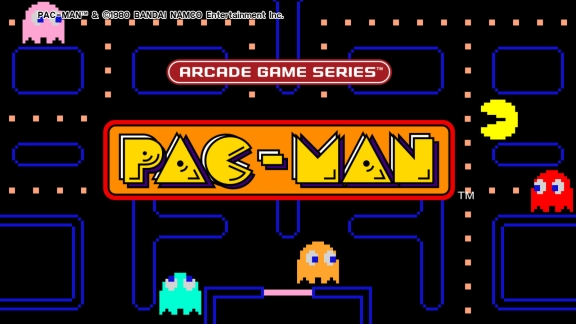
\includegraphics[width=.9\linewidth]{./pacman.jpg}
\caption{Une capture de la version Linux. \label{fig-capture}}
\end{figure}

\section{Algorithme}
\label{sec:orgfa5aabd}
Les déplacements des fantômes obéissent à des formules compliquées : \(\cos(\phi + \pi) = \xi/6\) \cite{tao2016_AnalysisII}.

\bibliography{../../../../complete_biblio}
\bibliographystyle{apacite}
\end{document}